\chapter{Localization}

Let R be a commutative ring with identity but not a field.

\begin{recall}
    A subset $U \subseteq R$ is \emph{multiplicatively closed} if $1 \in U$ and for $u,v \in U$, $uv \in U$, 
\end{recall}

\begin{example}
    \begin{enumerate}
        \item $\{1,f,f^2,\cdots\} \subseteq R$ is multiplicatively closed for $f \in R$.
        \item $R^\times \subseteq R$ is multiplicatively closed.
        \item $R \setminus \ffp \subseteq R$ is multiplicatively closed for $\ffp \in \operatorname{Spec}(R)$.
        \item $1 + \ffa \subseteq R$ is multiplicatively closed for $\ffa \leq R$.
    \end{enumerate}
\end{example}

\noindent Let $U \subseteq R$ be multiplicatively closed.

\begin{recall} \label{defOfMultiplicativelyClosedSet}
    $U^{-1}R = \{\frac{r}{u} \mid r \in R, u \in U\}$, where $\frac{r}{u} = \frac{r'}{u'}$ if and only if there exists $u'' \in U$ such that $u''(ru'-r'u) = 0$, i.e., $\frac{u''r}{u''u} = \frac{r'}{u'}$, formally, $\frac{r}{u}$ is the equivalence class under an equivalence relation. \par 
    $U^{-1}R$ is a commutative ring with identity with $\frac{r}{u} + \frac{s}{v} = \frac{rv+su}{uv}$ and $\frac{r}{u} \frac{s}{v} = \frac{rs}{uv}$ for $\frac{r}{u},\frac{s}{v} \in U^{-1}R$. \par 
    $0_{U^{-1}R} = \frac{0_R}{1_R} = \frac{0}{u}$ and $1_{U^{-1}R} = \frac{1_{R}}{1_{R}} = \frac{u}{u}$ for all $u \in U$. \par 
    $\frac{r}{u} = 0$ if and only if there exists $u'' \in U$ such that $u''r = 0$. \par 
    $\psi: R \to U^{-1}R$ given by $\psi(r) = \frac{r}{1}$ is a well-defined ring homomorphism. $\psi$ is 1-1 if and only if $U$ has no zero divisors.
\end{recall}

\begin{notation}
    \begin{enumerate}
        \item If $U = \{1,f,f^2,\cdots\}$, write $U^{-1}R = R_f$.
        \item If $U = R \setminus \ffp$ for some $\ffp \in \operatorname{Spec}(R)$, write $U^{-1}R = R_\ffp$.
        \item If $U \subseteq R$ is multiplicatively closed, write $U^{-1}R = R_U = R[U^{-1}]$.
    \end{enumerate}
\end{notation}

\noindent Let $\psi: R \to U^{-1}R$ be the natural ring homomorphism.

\begin{customrecall}{\ref{defOfMultiplicativelyClosedSet}+$\epsilon$}
    For $u \in U$, $\psi(u) \in (U^{-1}R)^{\times}$ since $\frac{1}{u} = (\frac{u}{1})^{-1} = (\psi(u))^{-1}$. So localization makes more elements invertible.
\end{customrecall}

\noindent Let $\varphi: R \to S$ be a ring homomorphism. 

\begin{proposition}[UMP for $\psi$]
    Let $\varphi(U) \subseteq S^{\times}$. Then there exists a unique ring homomorphism $\Phi:U^{-1}R \to S$ such that $\Phi \circ \psi = \varphi$. In fact, $\Phi(\frac{r}{u}) = \varphi(r)\varphi(u)^{-1}$ for $\frac{r}{u} \in U^{-1}R$.
    \begin{center}
        \begin{tikzcd}
            R \rar["\psi"] \drar["\varphi"'] & U^{-1}R \dar[dashed,"\ex !\ \Phi"] \\
            & S
        \end{tikzcd}
        \ \ \ \ \ \ 
        \begin{tikzcd}
            R \rar["\psi"] \drar["\varphi"'] & U^{-1}R \dar["\Lambda"] \\
            & S
        \end{tikzcd}
    \end{center}
\end{proposition}

\begin{proof}
    Let $\frac{r}{u} = \frac{r'}{u'}$. Then there exists $u'' \in U$ such that $u''(ru'-r'u) = 0$. Since $\varphi$ is a ring homomorphism, we have $\varphi(u'')(\varphi(r)\varphi(u') - \varphi(r')\varphi(u)) = 0$. Also, since $\varphi(u'') \in S^{\times}$, we have $\varphi(r)\varphi(u') = \varphi(r')\varphi(u)$, i.e., $\varphi(r)\varphi(u)^{-1} = \varphi(r')\varphi(u')^{-1}$ since $\varphi(u), \varphi(u') \in S^{\times}$. So $\phi$ is well-defined. Since $\Phi(\frac{r}{u} + \frac{s}{v}) = \Phi(\frac{rv+su}{uv}) = \varphi(rv+su)\varphi(uv)^{-1} = (\varphi(r)\varphi(v) + \varphi(s)\varphi(u))) \varphi(u)^{-1}\varphi(v)^{-1} = \varphi(r)\varphi(u)^{-1} + \varphi(s)\varphi(v)^{-1} = \Phi(\frac{r}{u}) + \Phi(\frac{s}{v})$ and similarly, $\Phi(\frac{r}{u} \cdot \frac{s}{v}) = \Phi(\frac{r}{u})\Phi(\frac{s}{v})$ for $\frac{r}{u},\frac{s}{v} \in U^{-1}R$, we have $\Phi$ is a ring homomorphism. \par 
    Suppose there is another ring homomorphism $\Lambda: U^{-1}R \to S$ such that $\Lambda \circ \psi = \varphi$.
    Then $\varphi(r) = \Lambda (\psi(r)) = \Lambda (\frac{r}{1})$ for $r \in R$. So $\Lambda(\frac{r}{u}) = \Lambda(\frac{r}{1} \frac{1}{u}) = \Lambda(\frac{r}{1}) \Lambda(\frac{u}{1})^{-1} = \varphi(r) \varphi(u)^{-1} = \Phi(\frac{r}{u})$ for $\frac{r}{u} \in U^{-1}R$. Thus, $\Lambda = \Phi$. 
\end{proof}

\begin{proposition}
    \begin{enumerate}
        \item $\varphi(U) \subseteq S$ is multiplicatively closed and $\varphi(U)^{-1}S =: U^{-1}S$.
        \item There is a ring homomorphism: $U^{-1}\varphi: U^{-1}R \to U^{-1}S$ given by $U^{-1}\varphi(r/u) = \varphi(r)/\varphi(u)$.
            \begin{center}
                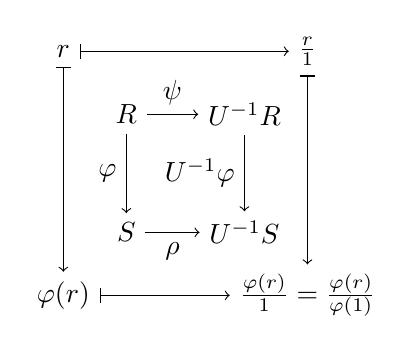
\begin{tikzpicture}[node distance = 1.5cm, auto]
                    \node (R) {$R$};
                    \node (UR)[right of=R] {$U^{-1}R$};
                    \node (S)[below of=R] {$S$};
                    \node (US)[below of=UR] {$U^{-1}S$};
                    \node (r)[node distance=0.8cm, left of=R, above of=R] {$r$};
                    \node (ur)[node distance=0.8cm, right of=UR, above of=UR] {$\frac{r}{1}$};
                    \node (s)[node distance=0.8cm, left of=S, below of=S] {$\varphi(r)$};
                    \node (us)[node distance=0.8cm, right of=US, below of=US] {$\frac{\varphi(r)}{1} = \frac{\varphi(r)}{\varphi(1)}$};
                    \draw[->] (R) to node {$\psi$} (UR);
                    \draw[->] (R) to node [swap]{$\varphi$} (S);
                    \draw[->] (UR) to node [swap] {$U^{-1}\varphi$} (US);
                    \draw[->] (S) to node [swap]{$\rho$} (US);
                    \draw[|->] (r) to node {} (ur);
                    \draw[|->] (r) to node {} (s);
                    \draw[|->] (s) to node {} (us);
                    \draw[|->] (ur) to node {} (us);
                \end{tikzpicture}
            \end{center}
        \item If $\varphi$ is onto, $U^{-1}\varphi$ is onto.
        \item If $\varphi$ is 1-1, $U^{-1}\varphi$ is 1-1.
        \item If $\alpha: S \to T$ is a ring homomorphism, then $U^{-1}(\alpha \circ \varphi) = (\varphi(U)^{-1}\alpha) \circ (U^{-1}\varphi)$. 
        \begin{center}
            \begin{tikzpicture}[node distance = 1.5cm, auto]
                \node (S) {$S$};
                \node (US)[node distance=3cm, right of=S] {$U^{-1}S$};
                \node (R)[above of=S, left of=S] {$R$};
                \node (T)[below of=S, left of=S] {$T$};
                \node (UR)[above of=S, right of=S] {$U^{-1}R$};
                \node (UT)[below of=S, right of=S] {$\varphi(U)^{-1}T$};

                \node [node distance=2cm, right of=UT] {$:=\alpha (\varphi(U))^{-1}T$};
                \node [node distance=1.45cm, right of=US] {$:=\varphi(U)^{-1}S$};
                \draw[->] (R) to node {$\varphi$} (S);
                \draw[->] (R) to node [swap]{$\alpha \circ \varphi$} (T);
                \draw[->] (S) to node {$\alpha$} (T);
                \draw[->] (R) to node {$\psi$} (UR);
                \draw[->] (T) to node {} (UT);
                \draw[->] (UR) to node {$U^{-1}\varphi$} (US);
                \draw[->] (US) to node {} (UT);
                \node (zzz)[node distance=0.8cm, below of=US] {$\varphi(U)^{-1} \alpha$};
                \draw[->,name path=line 1] (S) to node {} (US);
                \path[name path=line 2] (UR) to node {} (UT);
                % find intersection of first and second line
                \path [name intersections={of = line 1 and line 2}];
                \coordinate (P)  at (intersection-1);

                % path a circle around this intersection for the arc
                \path[name path=circle] (P) circle(1.0mm);
                % find intersections of second line and circle
                \path [name intersections={of = circle and line 2}];
                \coordinate (I1)  at (intersection-1);
                \coordinate (I2)  at (intersection-2);
                % draw normal line segments
                \draw (UR) -- (I1);
                \draw[->] (I2) -- (UT);
                % draw arc at intersection
                \tkzDrawArc[color=black](P,I1)(I2);
            \end{tikzpicture}
        \end{center}
    \end{enumerate}
\end{proposition}

\begin{proof}
    \begin{enumerate}
        \item [(b)] 
            Let $\frac{r}{u} = \frac{r'}{u'} \in U^{-1}R$. Then there exists $u'' \in U$ such that $u''(ru'-r'u) = 0$. So there exists $\varphi(u'') \in \varphi(U)$ such that $\varphi(u'')(\varphi(r)\varphi(u') - \varphi(r')\varphi(u)) = 0$. Hence $\frac{\varphi(r)}{\varphi(u)} = \frac{\varphi(r')}{\varphi(u')} \in U^{-1}S$. So $U^{-1}\varphi$ is well-defined. Since $U^{-1}\varphi(\frac{r}{u} + \frac{s}{v}) = U^{-1}\varphi(\frac{rv+su}{uv}) = \frac{\varphi(rv+su)}{\varphi(uv)} = \frac{\varphi(r)\varphi(v)+\varphi(s)\varphi(u)}{\varphi(u)\varphi(v)} = \frac{\varphi(r)}{\varphi(u)}+\frac{\varphi(s)}{\varphi(v)} = U^{-1}\varphi(\frac{r}{u})+U^{-1}(\varphi)(\frac{s}{v})$ and similarly, $U^{-1}(\varphi)(\frac{r}{u} \cdot\frac{s}{v}) = U^{-1}\varphi(\frac{r}{u})U^{-1}\varphi(\frac{s}{v})$ for $\frac{r}{u},\frac{s}{v} \in U^{-1}R$. 
        \item [(c)]
            Assume $\varphi$ is onto. Let $\frac{s}{\varphi(u)} \in U^{-1}S$ with $s \in S$ and $u \in U$. Since $\varphi: R \to S$ is onto, there exists $r \in R$ such that $\varphi(r) = s$. Then $U^{-1}\varphi(\frac{r}{u}) = \frac{\varphi(r)}{\varphi(u)} = \frac{s}{\varphi(u)}$. 
        \item[(d)] Assume $\varphi$ is 1-1. Let $\frac{r}{u} \in U^{-1}R$ with $r \in R$ and $u \in U$. Then $\frac{r}{u} \in \ker(U^{-1}\varphi)$ if and only if $0 = U^{-1}\varphi(\frac{r}{u}) = \frac{\varphi(r)}{\varphi(u)}$ if and only if there exists $u'' \in U$ such that $0 = \varphi(u'')\varphi(r) = \varphi(u''r)$ if and only if there exists $u'' \in U$ such that $u''r = 0$ since $\varphi$ is 1-1 if and only if $\frac{r}{u} = 0$ in $U^{-1}R$. 
        \item[(e)] 
            Since $\varphi:R \to S$ and $\alpha: S \to T$ are ring homomorphisms, $\alpha \circ \varphi$ is a ring homomorphism. Since $(\alpha \circ \varphi)(U) = \alpha(\varphi(U)) \subseteq T$ is multiplicatively closed by (a), we have $U^{-1}(\alpha \circ \varphi)$ and $\varphi(U)^{-1}\alpha$ are well-defined. Then by the following commutative diagram, $U^{-1}(\alpha \circ \varphi) = (\varphi(U)^{-1}\alpha) \circ (U^{-1}\varphi)$. 
        \[
            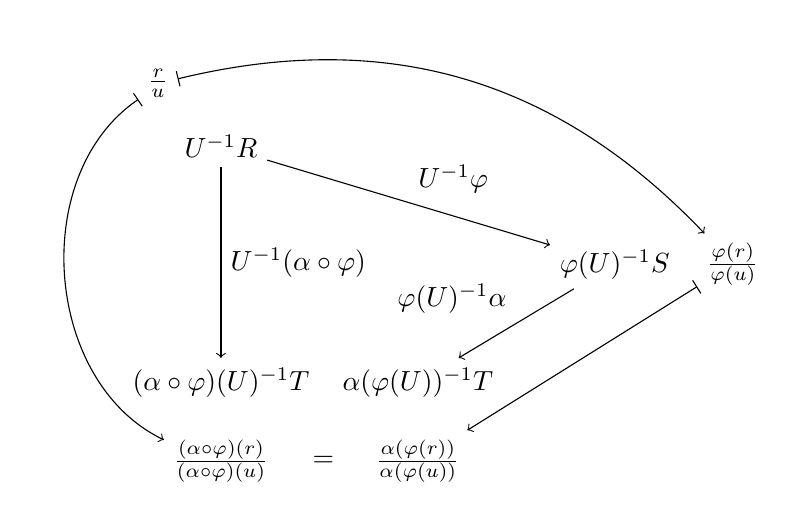
\begin{tikzpicture}[auto]
                \node (UR) {$U^{-1}R$};
                \node (UT)[node distance=3cm, below of=UR] {$(\alpha \circ \varphi)(U)^{-1}T$};
                \node (XXX)[node distance=1.5cm, below of=UR] {};
                \node (US)[node distance=5cm, right of=XXX] {$\varphi(U)^{-1}S$};
                \node (UT2)[node distance=2.5cm, right of=UT] {$\alpha (\varphi(U))^{-1}T$};
                \draw[->] (UR) to node {$U^{-1}(\alpha \circ \varphi)$} (UT);
                \draw[->] (UR) to node {$U^{-1}\varphi$} (US);
                \draw[->] (US) to node [swap]{$\varphi(U)^{-1}\alpha$} (UT2);
                \node (ur) [node distance=0.8cm, above of=UR,left of=UR]{$\frac{r}{u}$};
                \node (ut) [node distance=1cm, below of=UT]{$\frac{(\alpha \circ \varphi)(r)}{(\alpha \circ \varphi)(u)}$};
                \node (ut2) [node distance=1cm, below of=UT2]{$\frac{\alpha(\varphi(r))}{\alpha(\varphi(u))}$};
                \node (us) [node distance=1.5cm, right of=US]{$\frac{\varphi(r)}{\varphi(u)}$};
                \draw[|->, bend left] (ur) to node {} (us);
                \draw[|->] (us) to node [swap]{} (ut2);
                \draw[|->, bend right=60] (ur) to node {} (ut); 
                \node (equal) [node distance=1.3cm, right of=ut] {$=$}; 
            \end{tikzpicture} \qedhere
        \]
    \end{enumerate}
\end{proof}

\begin{proposition}
    Let $\varphi(U) \subseteq S$ be multiplicatively closed. Then $\im(U^{-1}\varphi) \cong U^{-1} \im(\varphi)$ given by $\frac{\varphi(r)}{\varphi(u)} \mapsto \frac{i(\pi(r))}{i(\pi(u))} = \frac{\varphi(r)}{\varphi(u)}$.
\end{proposition}

\begin{proof}
    We have 
    \begin{center}
        \begin{tikzpicture}[node distance = 1.6cm, auto]
            \node (Im) {$\im(\varphi)$};
            \node (UIm)[node distance=3cm, right of=Im] {$U^{-1}\im(\varphi)$};
            \node (R)[above of=Im, left of=Im] {$R$};
            \node (S)[below of=Im, left of=Im] {$S$};
            \node (UR)[above of=Im, right of=Im] {$U^{-1}R$};
            \node (US)[below of=Im, right of=Im] {$U^{-1}S$};
            \draw[->] (R) to node {$\pi$} (Im);
            \draw[->] (R) to node [swap]{$\varphi$} (S);
            \draw[->] (Im) to node {$i$} (S);
            \draw[->] (R) to node {$\psi$} (UR);
            \draw[->] (S) to node {} (US);
            \draw[->] (UR) to node {$U^{-1}\pi$} (UIm);
            \draw[->] (UIm) to node {} (US);
            \node (zzz)[node distance=0.85cm, below of=UIm] {$\pi(U)^{-1}i$};
            \node (www)[node distance=0.8cm, below of=UR] {};
            \node [node distance=0.55cm, left of=www] {$U^{-1}\varphi$};
            \draw[->,name path=line 1] (Im) to node {} (UIm);
            \path[name path=line 2] (UR) to node {} (US);
            % find intersection of first and second line
            \path [name intersections={of = line 1 and line 2}];
            \coordinate (P)  at (intersection-1);
            % path a circle around this intersection for the arc
            \path[name path=circle] (P) circle(1.0mm);
            % find intersections of second line and circle
            \path [name intersections={of = circle and line 2}];
            \coordinate (I1)  at (intersection-1);
            \coordinate (I2)  at (intersection-2);
            % draw normal line segments
            \draw (UR) -- (I1);
            \draw[->] (I2) -- (US);
            % draw arc at intersection
            \tkzDrawArc[color=black](P,I1)(I2);
        \end{tikzpicture}
    \end{center}
    By Proposition 3.6(e), $\im(U^{-1}\varphi) = \im(i \circ \pi) = \im((\pi(U)^{-1}i) \circ U^{-1}\pi)$. Since $\pi$ is onto, $U^{-1}(\pi)$ is onto by Proposition 3.6(c). So $\im(U^{-1}\varphi) = \im(\pi(U)^{-1}i)$. Since $i$ is 1-1, $\pi(U)^{-1}i$ is 1-1 by Proposition 3.6(d). Hence by the first isomorphism theorem, $U^{-1}\im(\varphi) \cong \im(\pi(U)^{-1}i) = \im(U^{-1}\varphi)$.
\end{proof}

\noindent Let $\ffa,\ffb \leq R$.

\begin{definition}
    Define a relation ``$\sim$'' on $U \times \ffa$ by $(u,a) \sim (u',a')$ if and only if there exists $u'' \in U$ such that $u''(u'a - ua') = 0$.
\end{definition}

\begin{fact}
    This is an equivalence relation.
\end{fact}

\begin{notation}
    $U^{-1}\ffa = \{\text{equivalence classes from $U \times \ffa$ under $\sim$}\}$, and $a/u$ or $\frac{a}{u}$ with $a \in \ffa$ and $u \in U$ are its elements, i.e., $U^{-1}\ffa = \{a/u \mid a \in \ffa, u \in U\}$.
\end{notation}

\begin{proposition}
    \begin{enumerate}
        \item The map $i: U^{-1}\ffa \to U^{-1}R$ given by $i(a/u) = a/u$ is a well-defined ring monomorphism. Identify $U^{-1}\ffa$ with $\im(i) \subseteq U^{-1}R$, so write $U^{-1}\ffa \subseteq U^{-1}R$. \par 
            \textbf{Warning.} $\frac{r}{u} \in U^{-1}R$ such that $\frac{r}{u} \in U^{-1}\ffa$ may have $r \not \in \ffa$.
        \item If $\frac{r}{u} \in U^{-1}R$, then $\frac{r}{u} \in U^{-1}\ffa$ if and only if there exists $v \in U$ such that $vr \in \ffa$, in this case, we have $\frac{r}{u} = \frac{vr}{vu} \in U^{-1}\ffa$ with $ur \in \ffa$ and $vu \in U$.
        \item Let $\pi: R \to \frac{R}{\ffa}$ be the natural surjection. Then $U^{-1}\ffa = \ker(U^{-1} \pi) \leq U^{-1}R$ and $\frac{U^{-1}R}{U^{-1}\ffa} \cong U^{-1}\frac{R}{\ffa} := \pi(U)^{-1} \frac{R}{\ffa}$.
        \item More generally, if $\varphi: R \to S$ is a ring homomorphism, then $U^{-1} \ker(\varphi) = \ker(U^{-1}\varphi) \leq U^{-1}R$ such that $\im(U^{-1}\varphi) \cong \frac{U^{-1}R}{U^{-1}\ker(\varphi)}$.
        \item $U^{-1}\ffa = \ffa \cdot U^{-1}R$, extension of $\ffa$ along $\psi: R \to U^{-1}R$.
    \end{enumerate}
\end{proposition}

\begin{proof}
    \begin{enumerate}
        \item By the definition of ``$\sim$'', $i$ is a well-defined ring monomorphism. Let $\frac{a}{u} \in U^{-1}\ffa$ with $a \in R$ and $u \in U$. Then $\frac{a}{u} \in \ker(i)$ if and only if $0 = i(\frac{a}{u}) = \frac{a}{u}$ in $U^{-1}R$ if and only if there exists $v \in U$ such that $va = 0 \in \ffa \subseteq R$ if and only if $\frac{a}{u} = \frac{va}{vu} = \frac{0}{vu} = 0$ in $U^{-1}\ffa$ by (b). Also, since $i$ is a ring homomorphism, $i$ is 1-1.
        \item Method 1. ``$\Rightarrow$''. Assume $\frac{r}{u} \in U^{-1}\ffa$. Then $\frac{r}{u} = \frac{a}{u'} \in U^{-1}R$ for some $a \in \ffa$ and $u \in U$. So there exists $u'' \in U$ such that $u''u'r = u''ua \in \ffa$ since $a \in \ffa$. Let $v = u''u'$. Then $vr = u''u'r \in \ffa$. \par 
            ``$\Leftarrow$''. Assume $vr \in \ffa$ for some $v \in U$. Then $\frac{r}{u} = \frac{vr}{vu} \in U^{-1}\ffa$. \par 
            Method 2. Note $\frac{r}{u} \in U^{-1}\ffa$ if and only if $\frac{r}{u} = \frac{a}{u'}$ for some $a \in \ffa$ and $u' \in U$ if and only if $u''u'r - u''ua = 0$ for some $a \in \ffa$ and $u', u'' \in U$ if and only if $1 \cdot v \cdot r - 1 \cdot 1 \cdot a = 0$ for some $a \in \ffa$ and $v \in U$ if and only if there exists $v \in U$ such that $vr \in \ffa$. 
        \item Note by Proposition 3.7, $\im(U^{-1}\pi) \cong U^{-1} \im(\pi) =  U^{-1}\frac{R}{\ffa}$ given by $\frac{\overbar{r}}{\overbar{u}} \mapsto \frac{\overbar{r}}{\overbar{u}}$. Then by (d), $U^{-1} \frac{R}{\ffa} \cong \frac{U^{-1}R}{U^{-1}\ker(\pi)} = \frac{U^{-1}R}{U^{-1}\ffa}$ given by $\frac{\overbar{r}}{\overbar{u}} \mapsfrom \overline{\frac{r}{u}}$.
        \item Let $\frac{r}{u} \in U^{-1}R$ with $r \in R$ and $u \in U$. Then $\frac{r}{u} \in U^{-1}\ker(\varphi)$ if and only if there exists $v \in U$ such that $vr \in \ker(\varphi)$ by (b) if and only if there exists $\varphi(v) \in \varphi(U)$ such that $0 = \varphi(vr) = \varphi(v)\varphi(r)$ if and only if $U^{-1}\varphi(\frac{r}{u}) = \frac{\varphi(r)}{\varphi(u)} = 0$ in $U^{-1}S = \varphi(U)^{-1}S$ if and only if $\frac{r}{u} \in \ker(U^{-1}\varphi)$. \par 
            By the first isomorphism theorem, $\im(U^{-1}\varphi) \cong \frac{U^{-1}R}{\ker(U^{-1}\varphi)} = \frac{U^{-1}R}{U^{-1}\ker(\varphi)}$ given by $\frac{\varphi(r)}{\varphi(u)} \mapsfrom \overline{\frac{r}{u}}$.  
            \begin{center}
                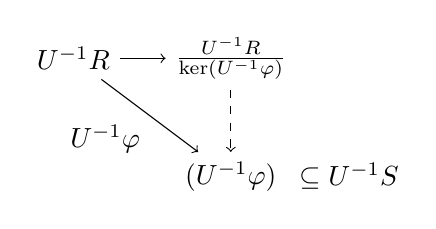
\begin{tikzpicture}[node distance=2cm,auto]
                    \node (UR) {$U^{-1}R$};
                    \node[right of=UR] (URK) {$\frac{U^{-1}R}{\ker(U^{-1}\varphi)}$};
                    \node[below of=URK, node distance=1.5cm] (US) {$\im(U^{-1}\varphi)$};
                    \node[right of=US,node distance=1.5cm] (xxx) {$\subseteq U^{-1}S$};
                    \draw[->] (UR) to node {} (URK); 
                    \draw[->] (UR) to node [swap] {$U^{-1}\varphi$} (US); 
                    \draw[->,dashed] (URK) to node {} (US); 
                \end{tikzpicture}
            \end{center}
        \item 
            ``$\supseteq$''. It follows from $\ffa \cdot U^{-1}R$ is generated by $\{\psi(a) = \frac{a}{1} \mid a \in \ffa\} \subseteq U^{-1}\ffa$. \par 
            ``$\subseteq$''. Let $\frac{a}{u} \in U^{-1}\ffa$ with $a \in \ffa$ and $u \in U$. Then $\frac{a}{u} = \frac{a}{1} \cdot \frac{1}{u} = \psi(a)\frac{1}{u} \in \ffa \cdot U^{-1}R$. \qedhere
    \end{enumerate}
\end{proof}

\begin{proposition}
    \begin{enumerate}
        \item $U^{-1}(\ffa + \ffb) = (U^{-1}\ffa) + (U^{-1}\ffb)$.
        \item $U^{-1}(\ffa \cap \ffb) = (U^{-1}\ffa) \cap (U^{-1}\ffb)$.
        \item $U^{-1}(\ffa \ffb) = (U^{-1}\ffa) (U^{-1}\ffb)$.
        \item $U^{-1} \operatorname{rad}(\ffa) = \operatorname{rad}(U^{-1}\ffa)$.
        \item $U^{-1}\operatorname{Nil}(R) = \operatorname{Nil}(U^{-1}R)$.
        \item $U^{-1}(\ffb:\ffa) = (U^{-1}\ffb:U^{-1}\ffa)$  if $\ffa$ is finitely generated.
    \end{enumerate}
\end{proposition}

\begin{proof}
    \begin{enumerate}
        \item By Proposition 3.11(e) and 1.63(c), we have $U^{-1}(\ffa+\ffb) = (\ffa+\ffb) \cdot U^{-1}R = (\ffa \cdot U^{-1}R) + (\ffb \cdot U^{-1}R) = (U^{-1}\ffa) + (U^{-1}\ffb)$.
        \item ``$\subseteq$''. By Proposition 3.11(e) and 1.63(d), $U^{-1}(\ffa \cap \ffb) = (\ffa \cap \ffb) \cdot U^{-1}R \subseteq (\ffa \cdot U^{-1}R) \cap (\ffb \cdot U^{-1}R) = (U^{-1}\ffa) \cap (U^{-1}\ffb)$. \par 
            ``$\supseteq$''. Let $\frac{r}{u} \in U^{-1}R$ with $r \in R,u \in U$ such that $\frac{r}{u} \in (U^{-1}\ffa) \cap (U^{-1}\ffb)$. Then there exist $v,w \in U$ such that $vr \in \ffa$ and $wr \in \ffb$ by Proposition 3.11(b). So $(vw)r \in \ffa \cap \ffb$. Also, since $vw \in U$, $\frac{r}{u} \in U^{-1}(\ffa \cap \ffb)$ by Proposition 3.11(b). \par
        \item By Proposition 3.11(e) and 1.63(e), we have $U^{-1}(\ffa\ffb) = (\ffa\ffb) \cdot U^{-1}R = (\ffa \cdot U^{-1}R)(\ffb \cdot U^{-1}R) = (U^{-1}\ffa)(U^{-1}\ffb)$.
        \item ``$\subseteq$''. By Proposition 3.11(e) and 1.63(g), $U^{-1} \operatorname{rad}(\ffa) = \operatorname{rad}(\ffa) \cdot U^{-1}R \subseteq \operatorname{rad}(\ffa \cdot U^{-1}R) = \operatorname{rad}(U^{-1}\ffa)$. \par 
            ``$\supseteq$''. Let $\frac{r}{u} \in \operatorname{rad}(U^{-1}\ffa)$ with $r \in R$ and $u \in U$. Then $\frac{r^{n}}{u^{n}} = (\frac{r}{u})^{n} \in U^{-1}\ffa$ for some $n \geq 1$. So there exists $v \in U$ such that $vr^{n} \in \ffa$ by Proposition 3.11(b). Hence $(vr)^{n} = v^{n-1} \cdot vr^{n} \in \ffa$. So $vr \in \operatorname{rad}(\ffa)$. Thus, $\frac{r}{u} \in U^{-1} \operatorname{rad}(\ffa)$ by Proposition 3.11(b).
        \item Special case of (d) with $\ffa = 0$. 
        \item ``$\subseteq$''. By Proposition 3.11(e) and 1.63(f), $U^{-1}(\ffb:\ffa) = (\ffb:\ffa) \cdot U^{-1}R \subseteq (\ffb \cdot U^{-1}R: \ffa \cdot U^{-1}R) = (U^{-1}\ffb:U^{-1}\ffa)$. \par 
            ``$\supseteq$''. Let $\frac{r}{u} \in U^{-1}R$ with $r \in R,u \in U$ such that $\frac{r}{u} \in (U^{-1}\ffb:U^{-1}\ffa)$. Since $\ffa$ is finitely generated, $\ffa = \langle a_{1},\cdots,a_{n} \rangle R$ for some $n \geq 1$ and $a_{1},\cdots,a_{n} \in R$. Then $U^{-1}\ffa = \langle \frac{a_{1}}{1},\cdots,\frac{a_{n}}{1} \rangle U^{-1}R$. Since $\frac{r}{u} \in (U^{-1}\ffb:U^{-1}\ffa)$, $\frac{ra_{i}}{u} = \frac{r}{u} \frac{a_{i}}{1} \in U^{-1}\ffb$ for $i = 1,\cdots,n$. So by Proposition 3.11(b), there exists $v_{i} \in U$ such that $v_{i} ra_{i} \in \ffb$ for $i = 1,\cdots,n$. Let $v = v_{1} \cdots v_{n} \in U$. Then $(vr)a_{i} \in \ffb$ for $i = 1,\cdots,n$. So $vr \in (\ffb:\ffa)$. Thus, $\frac{r}{u} \in U^{-1}(\ffb:\ffa)$ by Proposition 3.11(b). \qedhere
    \end{enumerate}
\end{proof}

\begin{proposition}
    \begin{enumerate}
        \item For $I \leq U^{-1}R$, there exists $\ffa \leq R$ such that $I = U^{-1}\ffa$, i.e., every ideal of $U^{-1}R$ is an extension of an ideal of $R$ along $\psi$.
        \item If $\ffa \leq R$, then $\psi^{-1}(U^{-1}\ffa) =\{r \in R \mid \ex v \in U \text{ s.t. }v r \in \ffa\} = \bigcup_{v \in U} (\ffa:v)$.
        \item $U^{-1}\ffa = U^{-1}R$ if and only if $U \cap \ffa \neq \emptyset$.
    \end{enumerate}
\end{proposition}

\begin{proof}
    \begin{enumerate}
        \item Since $I \leq U^{-1}R$, we have $\psi^{-1}(I) \leq R$. Claim. $I = U^{-1} (\psi^{-1}(I))$. \par 
            ``$\supseteq$''. By Proposition 1.63(a), $I \supseteq \psi^{-1}(I) \cdot U^{-1}R  = U^{-1} (\psi^{-1}(I))$. \par  
            ``$\subseteq$''. Let $i \in I$. Then $i = \frac{r}{u}$ for some $r \in R$ and $u \in U$. Also, since $\frac{u}{1} \in R$, $\psi(r) = \frac{r}{1} = \frac{r}{u} \cdot \frac{u}{1} \in I$, i.e., $r \in \psi^{-1}(I)$. So $i = \frac{r}{u} \in U^{-1} (\psi^{-1}(I))$.
        \item  
            Let $r \in R$. Then $r \in \psi^{-1}(U^{-1}\ffa)$ if and only if $\frac{r}{1} = \psi(r) \in U^{-1}\ffa$ if and only if $vr \in \ffa$ for some $v \in U$ by Proposition 3.11(b) if and only if $r \in (\ffa:v)$ for some $v \in U$ if and only if $r \in \bigcup_{v \in U}(\ffa:v)$. 
        \item
            Note $U^{-1}\ffa = U^{-1}R$ if and only if $\frac{1}{1} \in U^{-1}\ffa$ if and only if $1 \in \psi^{-1}(U^{-1}\ffa) = \bigcup_{v \in U}(\ffa:v)$ if and only if $U \cap \ffa \neq \emptyset$ by (b). \qedhere
    \end{enumerate}
\end{proof}

\begin{corollary}
    Let $\ffp \in \operatorname{Spec}(R)$ and $Q(R/\ffp)$ be the field of fraction. Then $R_\ffp = U^{-1}R$ is local with maximal ideal $\ffp_\ffp := \ffp R_{\ffp} = U^{-1}\ffp$ and $Q(R/\ffp) \xleftarrow \cong R_\ffp/\ffp_\ffp$ given by $\overbar r / \overbar u \mapsfrom \overbar {r/u}$.
\end{corollary}

\begin{proof} 
    Note $I \lneq U^{-1}R$ if and only if there exists $\ffa \lneq R$ with $U \cap \ffa = \emptyset$ such that $I = U^{-1}\ffa$ by Proposition 3.13(a) and (c). Since $\max\{\ffa \lneq R \mid U \cap \ffa = \emptyset\} = \ffp$, $\operatorname{m-Spec}(R_\ffp) = \{U^{-1}\ffp\}$. \par 
    Let $\tau: R \to R/\ffp$ be the natural projection. Then by Proposition 3.11(c), $R_{\ffp}/\ffp_{\ffp} = \frac{U^{-1}R}{U^{-1}\ffp} \cong U^{-1} \frac{R}{\ffp} := \tau(U)^{-1} \frac{R}{\ffp} = Q(R/\ffp)$.
\end{proof}

\begin{corollary}
    If $\ffm \in \operatorname{m-Spec}(R)$, then $R_\ffm/\ffm_\ffm \cong R/\ffm$.
\end{corollary}

\begin{proof}
    Since $\ffm \in \operatorname{m-Spec}(R)$, $R/\ffm$ is a field. So by Corollary 3.14, $R_\ffm/\ffm_\ffm \cong Q(R/\ffm) = R/\ffm$.
\end{proof}

\begin{example*}
    \begin{enumerate}
        \item Let $p \in \bbZ$ be prime. Then $\langle p \rangle \in \operatorname{m-Spec}(\bbZ)$. So $\bbZ_{(p)}/(p)_{(p)} \cong \bbZ/p\bbZ = \bbF_p$.
        \item 
            Let $a_1,\cdots,a_d \in k$. Then, similarly, $\frac{k[X_1,\cdots,X_d]_{(X_1-a_1,\cdots,X_d-a_d)}}{(X_1-a_1,\cdots,X_d-a_d)_{(X_1-a_1,\cdots,X_d-a_d)}} \cong Q(\frac{k[X_1,\cdots,X_d]}{(X_1-a_1,\cdots,X_d-a_d)}) \cong Q(k) = k$. 
    \end{enumerate}
\end{example*}

\noindent Let $\ffp \in \operatorname{Spec}(R)$. 

\begin{question*}
    $U \cap \ffp = \emptyset$ if and only if $U^{-1}\ffp \in \operatorname{Spec}(U^{-1}R)$ by prime correspondence for localization. What does $(U^{-1}R)_{U^{-1}\ffp}$ look like?
\end{question*}

\begin{lemma}
    Let $U \cap \ffp = \emptyset$. Let $\frac{r}{u} \in U^{-1}R$. Then $\frac{r}{u} \in U^{-1}\ffp$ if and only if $r \in \ffp$. 
\end{lemma}

\begin{proof}
    ``$\Leftarrow$''. By definition. \par 
    ``$\Rightarrow$''. Assume $\frac{r}{u} \in U^{-1}\ffp$. Then there exists $v \in U$ such that $vr \in \ffp \in \operatorname{Spec}(R)$. So $v \in \ffp$ or $r \in \ffp$. Since $v \in U$ and $U \cap \ffp = \emptyset$, we have $v \not \in \ffp$. So $r \in \ffp$.
\end{proof}

\begin{proposition}
    Let $U \cap \ffp = \emptyset$. Then $U^{-1}\ffp \in \operatorname{Spec}(U^{-1}R)$ and 
    \begin{align*}
        (U^{-1}R)_{U^{-1}\ffp} &\xrightarrow \cong R_\ffp \\
        \frac{r/1}{s/1} &\mapsfrom r/s \ s \in R \setminus \ffp 
    \end{align*}
\end{proposition}

\begin{proof}
    We have 
    \begin{center}
        \begin{tikzpicture}[node distance = 1.5cm, auto]
            \node (R) {$R$};
            \node (Rp)[right of=R,node distance = 2.5cm] {$R_\ffp$};
            \node (UR)[below of=R] {$U^{-1}R$};
            \node (URUp)[below of=Rp] {$(U^{-1}R)_{U^{-1}\ffp}$};
            \node (r)[node distance=0.8cm, left of=R, above of=R] {$r$};
            \node (rp)[node distance=0.8cm, right of=Rp, above of=Rp] {$\frac{r}{1}$};
            \node (ur)[node distance=0.8cm, left of=UR, below of=UR] {$r/1$};
            \node (urup)[node distance=0.8cm, right of=URUp, below of=URUp] {$\frac{r/1}{1/1}$};
            \draw[->] (R) to node {} (Rp);
            \draw[->] (R) to node [swap]{$\psi$} (UR);
            \draw[->] (R) to node {$\beta$} (URUp);
            \draw[->,dashed] (Rp) to node  {$\ex \varphi$} (URUp);
            \draw[->] (UR) to node [swap]{$\alpha$} (URUp);
            \draw[|->] (r) to node {} (rp);
            \draw[|->] (r) to node {} (ur);
            \draw[|->] (ur) to node {} (urup);
            \draw[|->,bend left] (rp) to node {} (urup);
        \end{tikzpicture}
    \end{center}
    Let $\beta = \alpha \circ \psi$. By proposition 3.5, to show $\varphi$ is a well-defined ring homomorphism, it suffices to show $\beta(R \setminus \ffp) \subseteq ((U^{-1}R)_{U^{-1}\ffp})^{\times}$ since $U \subseteq R \setminus \ffp$. Let $x \in R \setminus \ffp$. Then $\beta(x) = \frac{x/1}{1/1}$. Since $x/1 \in U^{-1}R$ and $x \not \in \ffp$, we have $x/1 \not \in U^{-1}\ffp$ by Lemma 3.16. So $\frac{x}{1}$ is an allowable denominator in $(U^{-1}R)_{U^{-1}\ffp}$. Hence $\frac{1/1}{x/1} \in (U^{-1}R)_{U^{-1}\ffp}$. Thus, $\frac{x/1}{1/1} \in ((U^{-1}R)_{U^{-1}\ffp})^{\times}$ with $(\frac{x/1}{1/1})^{-1} = \frac{1/1}{x/1}$. Besides, by Proposition 3.5, we have $\varphi(r/s) = \beta(r)/\beta(s) = \frac{r/1}{s/1}$ for $\frac{r}{s} \in R_\ffp$. \par 
    Let $\frac{r}{s} \in R_\ffp$. Then $\frac{r}{s} \in \ker(\varphi)$ if and only if $0 = \varphi(\frac{r}{s}) = \frac{r/1}{s/1} \in (U^{-1}R)_{U^{-1}\ffp}$ if and only if there exists $\frac{t}{v} \in U^{-1}R \setminus U^{-1}\ffp$ with $t \in R \setminus \ffp$ such that $\frac{tr}{v} = \frac{t}{v} \cdot \frac{r}{1} = 0$ in $U^{-1}R$ by Proposition 3.11(b) and Lemma 3.16 if and only if there exist $t \in R \setminus \ffp$ and $w \in U \subseteq R \setminus \ffp$ such that $wtr = 0$ in $R$ by Proposition 3.11(b) if and only if there exists $v' \in U \subseteq R \setminus \ffp$ such that $v'r = 0$ in $R$ since $R \setminus \ffp$ is multiplicatively closed if and only if $\frac{r}{s} = 0$ in $R_\ffp$ by Proposition 3.11(b). So $\varphi$ is 1-1. \par 
    Let $\frac{r/u}{s/v} \in (U^{-1}R)_{U^{-1}\ffp}$ with $r \in R$, $u,v \in U \subseteq R \setminus \ffp$ and $s \in R \setminus \ffp$. Then $us \in R \setminus \ffp$ since $R \setminus \ffp$ is multiplicatively closed. So $\frac{vr}{us} \in R_\ffp$. Also, since $\varphi(\frac{vr}{us}) = \frac{\beta(vr)}{\beta(us)} = \frac{vr/1}{us/1} = \frac{uv/1 \cdot r/u}{uv/1 \cdot s/v} = \frac{r/u}{s/v}$, we have $\varphi$ is onto. 
\end{proof}

\begin{corollary}
    If $\ffq \in \operatorname{Spec}(R)$ with $\ffp \subseteq \ffq$, then $\ffp_\ffq \in \operatorname{Spec}(R_\ffq)$ and $(R_\ffq)_{\ffp_\ffq} \xleftarrow \cong R_\ffp$ given by $\frac{r/1}{s/1} \mapsfrom r/s$.
\end{corollary}

\begin{proof}
    Take $U = R \setminus \ffq$ in Proposition 3.17.
\end{proof}

\begin{example*}
    \begin{enumerate}
        \item Let $0 \neq p \in \bbZ$ be prime. Then $(0) \subseteq (p) \subsetneq \bbZ$ and $\bbZ_{(p)}$ is a domain. So by Corollary 3.18, $Q(\bbZ_{(p)}) = (\bbZ_{(p)})_{(0)_{(p)}} \cong \bbZ_{(0)} = Q(\bbZ) = \bbQ$. 
        \item Let $R$ be a domain and $0 \not \in U$. Then $U^{-1}R$ is a domain and $\ffp := (0) \in \operatorname{Spec}(R)$. So $Q(U^{-1}R) = (U^{-1}R)_{U^{-1}(0)} \cong R_{(0)} = Q(R)$ by Proposition 3.17. In fact, the map $Q(U^{-1}R) \xleftarrow \cong Q(R)$ is given by $\frac{r/1}{s/1} \mapsfrom r/s$.
    \end{enumerate}
\end{example*}

\begin{proposition}
    Let $R \neq 0$. Then $\operatorname{NZD}(R) \subseteq R$ is multiplicatively closed. Moreover, it is \emph{saturated}: if $r,s \in R$ such that $rs \in \operatorname{NZD}(R)$, then $r,s \in \operatorname{NZD}(R)$. 
\end{proposition}

\begin{proof}
    Since $R \neq 0$, $1 \in \operatorname{NZD}$. Let $r,s \in \operatorname{NZD}(R)$. Assume $(rs)t=0$ for some $t \in R$. Then $r(st) = 0$. Since $r \in \operatorname{NZD}(R)$, $st = 0$. Also, since $s \in \operatorname{NZD}(R)$, $t = 0$. So $rs \in \operatorname{NZD}(R)$. \par 
    Let $x,y \in R$ such that $xy \in \operatorname{NZD}(R)$. By symmetry, we need to show $x \in \operatorname{NZD}(R)$. Assume $xz = 0$ for some $z \in R$. Then $(xy)z = y(xz) = 0$. Since $xy \in \operatorname{NZD}(R)$, $z = 0$.
\end{proof}

\begin{definition}
    The \emph{total ring of fractions of} $R$ (or \emph{total quotient ring of }$R$) is $\operatorname{Q}(R) = \operatorname{NZD}(R)^{-1}R$.
\end{definition}

\begin{example*}
    \begin{enumerate}
        \item If $R$ is a domain, then $\operatorname{NZD}(R) = R \setminus \{0\}$ and $\operatorname{Q}(R) = \operatorname{NZD}(R)^{-1}(R) = (R \setminus 0)^{-1}(R) = Q(R)$. So the total ring of fractions of a domain is equal to the field of fraction. 
        \item Let $R = \frac{k[X,Y,Z,W]}{\langle XY,YZ,ZW,XW \rangle}$, not a domain. Let $G$ be the following graph: 
            \begin{center}
            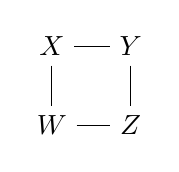
\begin{tikzpicture}[node distance=1cm]
                \node (X) {$X$}; 
                \node[right of=X] (Y) {$Y$}; 
                \node[below of=X] (W) {$W$}; 
                \node[right of=W] (Z) {$Z$};
                \draw (X) -- (Y);
                \draw (X) -- (W);
                \draw (Y) -- (Z);
                \draw (W) -- (Z);
            \end{tikzpicture}
            \end{center}
            Then the edge ideal of $G$ is $I_G = \langle XY,YZ,ZW,XW \rangle$. Let $P_V = \langle X \mid X \in V \rangle$ for $V \subseteq V(G)$. Then we have $I_G = \bigcap_{V\text{ min. v.cover}} P_V = P_{\{X,Z\}} \cap P_{\{Y,W\}} =\langle X,Z \rangle \cap \langle Y,W \rangle$. So $\operatorname{Min}(k[X,Y,Z,W]) = \{P_V \mid V\text{ min. v.cover}\} = \{\langle X,Z \rangle, \langle Y,W \rangle\}$. By Fact 1.15, $\operatorname{Min}(R) = \{\langle \overbar{X},\overbar{Z} \rangle, \langle \overbar{Y}, \overbar{W} \rangle\}$. So $\operatorname{ZD}(R) = \bigcup_{\ffp \in \operatorname{Min}(R)}\ffp = \langle \overbar{X}, \overbar{Z} \rangle \cup \langle \overbar{Y}, \overbar{W} \rangle$. Then $U := \operatorname{NZD}(R) = R \setminus \{\langle \overbar{X}, \overbar{Z} \rangle \cup \langle \overbar{Y}, \overbar{W} \rangle\}$. \par 
            By prime correspondence for localization, $\operatorname{Spec}(\operatorname{Q}(R)) = \{U^{-1}\ffp \mid \ffp \in \operatorname{Spec}(R), \ffp \cap U = \emptyset\} = \{U^{-1}\langle \overbar{X}, \overbar{Z} \rangle, U^{-1}\langle \overbar{Y}, \overbar{W} \rangle\}$. Also, by Proposition 3.12(b), $U^{-1}\langle \overbar{X}, \overbar{Z} \rangle \cap U^{-1}\langle \overbar{Y}, \overbar{W} \rangle = U^{-1}(\langle \overbar{X}, \overbar{Z} \rangle \cap \langle \overbar{Y}, \overbar{W} \rangle) = U^{-1} \langle \overbar{XY,YZ,ZW,XW} \rangle = 0$. Therefore, $\operatorname{Min}(U^{-1}R) = \{U^{-1}\langle \overbar{X}, \overbar{Z}\rangle, U^{-1} \langle \overbar{Y}, \overbar{W} \rangle\} = \operatorname{m-Spec}(U^{-1}R)$. Since $R$ is reduced, $\operatorname{Nil}(R) = 0$ and then $\operatorname{Nil}(U^{-1}R) = U^{-1}\operatorname{Nil}(R) = 0$ by Proposition 3.12(e), i.e., $\operatorname{Q}(R)$ is reduced. So $\operatorname{ZD}(\operatorname{Q}(R)) = \bigcup_{\ffp \in \operatorname{Min}(\operatorname{Q}(R))}\ffp = U^{-1} \langle \overbar{X}, \overbar{Z} \rangle \cup U^{-1} \langle \overbar{Y}, \overbar{W} \rangle$. \par Let $\pi_1: R \to R/\langle \overbar{X}, \overbar{Z} \rangle$ and $\pi_2: R \to R/\langle \overbar{Y}, \overbar{W} \rangle$ be natural surjections. Then by Chinese Remainder Theorem and Proposition 3.17 with $0 \not \in \pi_1(R \setminus \langle \overbar{X}, \overbar{Z} \rangle \cup \langle \overbar{Y}, \overbar{W} \rangle) = \pi_1(U)$ and $0 \not \in \pi_2(U)$,
            \begin{align*}
                \operatorname{Q}(R) &\cong \frac{U^{-1}R}{(U^{-1}\langle \overbar{X},\overbar{Z} \rangle) \cap (U^{-1}\langle \overbar{Y},\overbar{W} \rangle)} \cong \frac{U^{-1}R}{U^{-1} \langle \overbar{X}, \overbar{Z} \rangle} \times \frac{U^{-1}R}{U^{-1} \langle \overbar{Y}, \overbar{W} \rangle} \cong U^{-1}\frac{R}{\langle \overbar{X}, \overbar{Z} \rangle} \times U^{-1} \frac{R}{\langle \overbar{Y}, \overbar{W} \rangle} \\
                &\cong Q\left(U^{-1}\frac{R}{\langle \overbar{X},\overbar{Z} \rangle}\right) \times Q\left(U^{-1}\frac{R}{\langle \overbar{Y},\overbar{W} \rangle}\right) \cong \left(U^{-1}\frac{R}{\langle \overbar{X}, \overbar{Z} \rangle} \right)_{U^{-1}(0)} \times \left(U^{-1}\frac{R}{\langle \overbar{Y}, \overbar{W} \rangle} \right)_{U^{-1}(0)} \\
                &\cong \left(\frac{R}{\langle \overbar{X}, \overbar{Z} \rangle}\right)_{(0)} \times \left(\frac{R}{\langle \overbar{Y},\overbar{W} \rangle}\right)_{(0)} \cong Q\left(\frac{R}{\langle \overbar{X},\overbar{Z} \rangle}\right) \times Q\left(\frac{R}{\langle \overbar{Y}, \overbar{W} \rangle}\right) \cong Q(k[Y,W]) \times Q(k[X,Z]).
            \end{align*}
            \begin{comment}
            \par Let $R_1: = \frac{R}{\langle \overbar{X}, \overbar{Z} \rangle} \cong k[Y,W]$ and $R_2 := \frac{R}{\langle \overbar{Y}, \overbar{W} \rangle} \cong k[X,Z]$. Note $R_1$ is an integral domain and $U^{-1}R_1$ is a field. By UMP, there exists a unique ring homomorphism $\overbar{\varphi}_1$ such that the following diagram commutes. Also, since $\overbar{\varphi}_1 \neq 0$ and $\operatorname{Q}(R_1)$ is a field, $\overbar{\varphi}_1$ is 1-1. Let $\frac{r}{u} \in U^{-1}R_1$ with $r \in R$ and $u \in \pi_1(U) = \pi_1(R \setminus (\langle \overbar{X},\overbar{Z} \rangle \cup \langle \overbar{Y}, \overbar{W} \rangle)) \subseteq R_1 \setminus \{0\}$. Then $\frac{r}{u} \in \operatorname{Q}(R_1)$. Since $\overbar{\varphi}_1(\frac{r}{u}) = \frac{\varphi_1(r)}{\varphi_1(u)} = \frac{r/1}{u/1} = \frac{r}{u}$, we have $\overbar{\varphi_1}$ is onto. Hence $\operatorname{Q}(R_1) \cong U^{-1}R_1$. Similarly, $\operatorname{Q}(R_2) \cong U^{-1}R_2$.
             \begin{center}
                \begin{tikzpicture}[node distance = 1.5cm, auto]
                    \node (R) {$R_1$};
                    \node (QR)[right of=R] {$\operatorname{Q}(R_1)$};
                    \node (L)[below of=QR] {$U^{-1}R_1$};
                    \node (r)[node distance=0.7cm, left of=R, above of=R] {$r_1$};
                    \node (qr)[node distance=0.7cm, right of=QR, above of=QR] {$\frac{r_1}{1}$};
                    \node (qru)[node distance=1.6cm, right of=QR] {$\frac{r_1}{u_1}$};
                    \node (lu)[below of=qru] {$\frac{\varphi_1(r_1)}{\varphi_1(u_1)}$};
                    \node (l)[node distance=0.7cm, below of=L] {$r_1/1 = \frac{r_1/1}{1/1}$};
                    \draw[->] (R) to node {$\psi_1$} (QR);
                    \draw[right hook->] (R) to node [swap]{$\varphi_1$} (L);
                    \draw[->,dashed] (QR) to node {$\ex !\ \overbar \varphi_1$} (L);
                    \draw[|->] (r) to node {} (qr);
                    \draw[|->,bend right] (r) to node {} (l);
                    \draw[|->,bend left=45] (qr) to node {} (l);
                    \draw[|->] (qru) to node {} (lu);
                \end{tikzpicture}
                \ \ \ \ \ \ 
                \begin{tikzpicture}[node distance = 1.5cm, auto]
                    \node (R) {$R_2$};
                    \node (QR)[right of=R] {$\operatorname{Q}(R_2)$};
                    \node (L)[below of=QR] {$U^{-1}R_2$};
                    \node (r)[node distance=0.7cm, left of=R, above of=R] {$r_2$};
                    \node (qr)[node distance=0.7cm, right of=QR, above of=QR] {$\frac{r_2}{1}$};
                    \node (qru)[node distance=1.6cm, right of=QR] {$\frac{r_2}{u_2}$};
                    \node (lu)[below of=qru] {$\frac{\varphi_2(r_2)}{\varphi_2(u_2)}$};
                    \node (l)[node distance=0.7cm, below of=L] {$r_2/1 = \frac{r_2/1}{1/1}$};
                    \draw[->] (R) to node {$\psi_2$} (QR);
                    \draw[right hook->] (R) to node [swap]{$\varphi_2$} (L);
                    \draw[->,dashed] (QR) to node {$\ex !\ \overbar \varphi_2$} (L);
                    \draw[|->] (r) to node {} (qr);
                    \draw[|->,bend right] (r) to node {} (l);
                    \draw[|->,bend left=45] (qr) to node {} (l);
                    \draw[|->] (qru) to node {} (lu);
                \end{tikzpicture}
            \end{center}
            Thus, $\operatorname{Q}(R) \cong \operatorname{Q}(R/\langle \overbar{X}, \overbar{Z} \rangle) \times \operatorname{Q}(R/\langle \overbar{Y}, \overbar{W} \rangle) \cong \operatorname{Q}(k[Y,W]) \times \operatorname{Q}(k[X,Z]) \cong k(X,Z) \times k(Y,W)$ by (a).
        \end{comment}
    \end{enumerate}
\end{example*}

\begin{proposition}
    The natural ring homomorphism $\psi: R \to \operatorname{Q}(R)$ is 1-1. Moreover, $\operatorname{NZD}(R)$ is the unique largest multiplicatively closed subset of $R$ with this property.
\end{proposition}

\begin{proof}
    Let $r \in R$. Then $r \in \ker(\psi)$ if and only if $\psi(r) = 0 = \frac{r}{1}$ in $\operatorname{Q}(R)$ if and only if there exists $v \in \operatorname{NZD}(R)$ such that $vr = 0$ by Proposition 3.11(b) if and only if $r = 0$. So $\psi$ is 1-1. \par
    Assume $U \subseteq R$ is multiplicatively closed such that the natural ring homomorphism $\phi: R \to U^{-1}R$ is 1-1. Let $u \in U$. Let $r \in R$ such that $ur = 0$. Then $\phi(r) = \frac{r}{1} = \frac{ur}{u} = \frac{0}{u} = 0$. Also, since $\phi$ is 1-1, $r = 0$. So $u \in \operatorname{NZD}(R)$.
\end{proof}

\begin{question}
    Let $\varphi^*: \operatorname{Spec}(S) \to \operatorname{Spec}(R)$.
    \begin{enumerate}
        \item When is $\ffp \in \im(\varphi^*)$?, i.e., when does there exist $\ffq \in \operatorname{Spec}(S)$ such that $\ffp  = \varphi^{-1}(\ffq)$.
        \item What does $(\varphi^*)^{-1}(\ffp) = \{\ffq \in \operatorname{Spec}(S) \mid \varphi^*(\ffq) = \ffp\}$ look like? In general, if $f: Y \to X$ is a (continuous) function and $x \in X$, then $f^{-1}(x) = \{y \in Y \mid f(y) = x\} = \text{fibre over $x$ w.r.t. $f$}$.
    \end{enumerate}
\end{question}

\begin{construction}
    Let $U = R \setminus \ffp$. 
    \begin{center}
        \begin{tikzpicture}[node distance=3cm,auto]
            \node (R) {$R$}; 
            \node[right of=R] (S) {$S$}; 
            \node[below of=R,node distance=1.3cm] (UR) {$U^{-1}R$}; 
            \node[below of=S,node distance=1.3cm] (US) {$U^{-1}S$}; 
            \node[below of=UR,node distance=1.5cm] (URpUR) {$\frac{U^{-1}R}{U^{-1}\ffp U^{-1}R}$}; 
            \node[below of=US,node distance=1.5cm] (USpUS) {$\frac{U^{-1}S}{\ffp \cdot U^{-1}S}$}; 
            \draw[->] (R) to node {$\varphi$} (S);
            \draw[->] (R) to node {$\psi$} (UR);
            \draw[->] (S) to node {$\rho$} (US);
            \draw[->] (UR) to node {$U^{-1}\varphi$} (US);
            \draw[->] (UR) to node {$\tau$} (URpUR);
            \draw[->] (US) to node {$\pi$} (USpUS);
            \draw[->] (URpUR) to node {$\overbar{\pi \circ U^{-1}\varphi}$} (USpUS);
            \node[left of=UR,node distance=0.98cm] (xxx) {$R_\ffp=$}; 
            \node[left of=URpUR,node distance=2.08cm] (yyy) {$Q(R/\ffp) \cong \frac{R_\ffp}{\ffp_\ffp}=$}; 
            \node[right of=USpUS,node distance=2.45cm] (zzz) {$:=\frac{U^{-1}S}{\ffp S \cdot U^{-1}S}:=\frac{U^{-1}S}{U^{-1}\ffp \cdot U^{-1}S}$}; 
            \node[below of=USpUS,node distance=0.9cm] (uuu) {$\llF(\ffp)$};
            \node[right of=uuu,node distance=2cm] (vvv) {$= \frac{S_\ffp}{\ffp \cdot S_\ffp} := \frac{\varphi(U)^{-1}S}{\varphi(U)^{-1}(\ffp S)}$};
            \node[right of=US,node distance=1.45cm] (www) {$:=\varphi(U)^{-1}S$}; 
            \draw[double equal sign distance] (USpUS) to node{} (uuu);
        \end{tikzpicture}
    \end{center}
    Note $\ffp \cdot U^{-1}S$ is the extension of $\ffp$ along $\rho \circ \varphi$, $\ffp S \cdot U^{-1}S$ is the extension of $\ffp S$ along $\rho$, and $U^{-1}\ffp \cdot U^{-1}S$ is the extension of $U^{-1}\ffp$ along $U^{-1}\varphi$. $\llF(\ffp)$ is fibre over $\ffp$ w.r.t. $\varphi$. \par 
    Let $\frac{p}{u} \in U^{-1}\ffp$ with $p \in \ffp$ and $u \in U$. Then $\pi \circ (U^{-1}\varphi)(\frac{p}{u})  = \pi(\frac{\varphi(p)}{\varphi(u)}) = 0$ in $\frac{\varphi(U)^{-1}S}{\varphi(U)^{-1}(\ffp S)}$ since $\varphi(p) \subseteq \ffp S$. So by Construction 1.13, $\overbar{\pi \circ (U^{-1}\varphi)}$ is a well-defined ring homomorphism.
    \begin{center}
        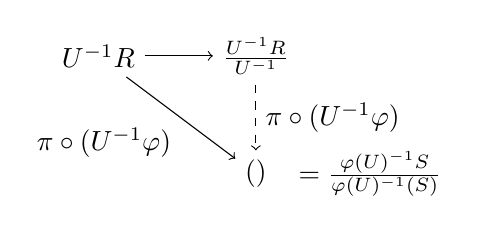
\begin{tikzpicture}[node distance=2cm,auto]
            \node (UR) {$U^{-1}R$};
            \node[right of=UR] (URK) {$\frac{U^{-1}R}{U^{-1}\ffp}$};
            \node[below of=URK, node distance=1.5cm] (Fp) {$\llF(\ffp)$};
            \node[right of=Fp, node distance=1.45cm] (xxx) {$=\frac{\varphi(U)^{-1}S}{\varphi(U)^{-1}(\ffp S)}$};
            \draw[->] (UR) to node {} (URK); 
            \draw[->] (UR) to node [swap] {$\pi \circ (U^{-1}\varphi)$} (Fp); 
            \draw[->,dashed] (URK) to node {$\overbar{\pi \circ (U^{-1}\varphi)}$} (Fp); 
        \end{tikzpicture}
    \end{center}
    \begin{center}
        \begin{tikzpicture}[node distance=1.1cm,auto]
            \node (R) {$R$};
            \node[right of=R,node distance=6cm] (S) {$S$};
            \node[left of=R,below of=R] (UR) {$U^{-1}R$};
            \node[right of=R,below of=R,node distance = 2cm] (Rp) {$\frac{R}{\ffp}$};
            \node[right of=S,below of=S,node distance = 2cm] (SpS) {$\frac{S}{\ffp S}$};
            \node[left of=S,below of=S] (US) {$U^{-1}S$};
            \node[left of=Rp,below of=Rp] (URpUR) {$\frac{U^{-1}R}{U^{-1}\ffp}$};
            \node[left of=Rp,below of=SpS] (USpUS) {$\frac{\varphi(U)^{-1}S}{\varphi(U)^{-1} (\ffp S)}$};
            \node[below of=US,node distance=0.4cm] (ttt) {};
            \node[right of=ttt,node distance=0.75cm] (tttt) {$\pi$};
            \draw[->] (R) to node {$\varphi$} (S);
            \draw[->] (R) to node [swap]{$\psi$} (UR);
            \draw[->] (S) to node {$\rho$} (US);
            \draw[->] (S) to node {$\epsilon$} (SpS);
            \draw[->] (UR) to node {$\tau$} (URpUR);
            \draw[->] (Rp) to node [swap] {$\overbar{\tau \circ \psi}$} (URpUR);
            \draw[->] (SpS) to node {} (USpUS);
            \node[below of=SpS,node distance=0.6cm] (mmm) {};
            \node[right of=mmm,node distance=0.2cm] (nnn) {$\overbar{\pi \circ \rho}$};
            \node[below of=US,node distance=0.65cm] (ooo) {};
            \node[left of=ooo,node distance=0.5cm] (ppp) {$\overbar{\epsilon \circ \varphi}$};
            \node[below of=R,node distance=0.8cm] (qqq) {};
            \node[right of=qqq,node distance=2.5cm] (fff) {$U^{-1}\varphi$};
            \draw[->] (URpUR) to node {$\overbar{\pi \circ (U^{-1}\varphi)}$} (USpUS);
            \draw[->,name path=line 1] (UR) to node {} (US);
            \path[name path=line 2] (R) to node {} (Rp);
            % find intersection of first and second line
            \path [name intersections={of = line 1 and line 2}];
            \coordinate (P)  at (intersection-1);

            % path a circle around this intersection for the arc
            \path[name path=circle] (P) circle(1.0mm);
            % find intersections of second line and circle
            \path [name intersections={of = circle and line 2}];
            \coordinate (I1)  at (intersection-1);
            \coordinate (I2)  at (intersection-2);
            % draw normal line segments
            \draw (R) -- (I1);
            \draw[->] (I2) -- (Rp);
            % draw arc at intersection
            \tkzDrawArc[color=black](P,I1)(I2);
            \draw[->,name path=line 1] (Rp) to node {} (SpS);
            \path[name path=line 2] (US) to node {} (USpUS);
            % find intersection of first and second line
            \path [name intersections={of = line 1 and line 2}];
            \coordinate (P)  at (intersection-1);

            % path a circle around this intersection for the arc
            \path[name path=circle] (P) circle(1.0mm);
            % find intersections of second line and circle
            \path [name intersections={of = circle and line 2}];
            \coordinate (I1)  at (intersection-1);
            \coordinate (I2)  at (intersection-2);
            % draw normal line segments
            \draw (US) -- (I1);
            \draw[->] (I2) -- (USpUS);
            % draw arc at intersection
            \tkzDrawArc[color=black](P,I1)(I2);
        \end{tikzpicture}
    \end{center}
    Let $\overbar{r} \in \frac{R}{\ffp}$ with $r \in R$. Then $\overbar{\pi \circ (U^{-1}\varphi)} \circ (\overbar{\tau \circ \psi})(\overbar{r}) = \overbar{\pi \circ (U^{-1}\varphi)}(\tau \circ \psi(r)) = \overbar{\pi \circ (U^{-1}\varphi)}\left(\overline{\frac{r}{1}}\right) = \pi \circ (U^{-1}\varphi)\left(\frac{r}{1}\right) = \overline{\frac{\varphi(r)}{\varphi(1)}} = \overline{\frac{\varphi(r)}{1}}$ and $\overbar{\pi \circ \rho} \circ \overbar{\epsilon \circ \varphi}(\overbar{r}) = \overbar{\pi \circ \rho}(\epsilon \circ \rho)(r) = \overbar{\pi \circ \rho}(\overbar{\phi(r)}) = \pi \circ \rho(\phi(r)) = \overline{\frac{\varphi(1)}{1}}$. So the diagram on the bottom also commutes.
\end{construction}

\begin{theorem}
    Let $\varphi^*: \operatorname{Spec}(S) \to \operatorname{Spec}(R)$ and $U = R \setminus \ffp$. Then the followings are equivalent.
    \begin{enumerate}
        \item[(i)] $\ffp \in \im(\varphi^*)$, i.e., $(\varphi^*)^{-1}(\ffp) \neq \emptyset$.
        \item[(ii)] $\ffp = \varphi^{-1}(\ffp S)$, where $\ffp S$ is not necessarily prime.
        \item[(iii)] $\ffp \cdot U^{-1}S \neq U^{-1}S$, i.e., $\llF(\ffp) = \frac{U^{-1}S}{\ffp \cdot U^{-1}S} \neq 0$.
    \end{enumerate}
    Moreover, the map $\theta: \operatorname{Spec}(\llF(\ffp)) \to (\varphi^*)^{-1}(\ffp) \subseteq \operatorname{Spec}(S)$ given by $\theta(Q) = \rho^{-1}(\pi^{-1}(Q))$ is a well-defined bijection, where $(\varphi^{*})^{-1}(\ffp)$ is the fibre over $\ffp$ w.r.t. $\varphi^{*}: \operatorname{Spec}(S) \to \operatorname{Spec}(R)$.
    \begin{center}
        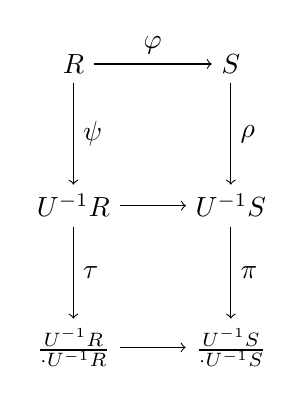
\begin{tikzpicture}[node distance=2cm,auto]
            \node (R) {$R$}; 
            \node[right of=R] (S) {$S$}; 
            \node[below of=R,node distance=1.8cm] (UR) {$U^{-1}R$}; 
            \node[below of=S,node distance=1.8cm] (US) {$U^{-1}S$}; 
            \node[below of=UR,node distance=1.8cm] (URpUR) {$\frac{U^{-1}R}{\ffp \cdot U^{-1}R}$}; 
            \node[below of=US,node distance=1.8cm] (USpUS) {$\frac{U^{-1}S}{\ffp \cdot U^{-1}S}$}; 
            \draw[->] (R) to node {$\varphi$} (S);
            \draw[->] (R) to node {$\psi$} (UR);
            \draw[->] (S) to node {$\rho$} (US);
            \draw[->] (UR) to node {} (US);
            \draw[->] (UR) to node {$\tau$} (URpUR);
            \draw[->] (US) to node {$\pi$} (USpUS);
            \draw[->] (URpUR) to node {} (USpUS);
        \end{tikzpicture}
    \end{center}

\end{theorem}

\begin{proof}
    ``(i)$\Rightarrow$(ii)''. Assume there is $\ffq \in \operatorname{Spec}(S)$ such that $\ffp = \varphi^*(\ffq)$. Then $\ffp = \varphi^{-1}(\ffq) = \varphi^{-1}(\varphi^{-1}(\ffq)S) = \varphi^{-1}(\ffp S)$ by 1.63(b). \par 
    ``(ii)$\Rightarrow$(iii)''. Assume $\ffp = \varphi^{-1}(\ffp S)$. Note $\ffp \cdot U^{-1}S = \ffp S \cdot U^{-1}S = \ffp S \cdot \varphi(U)^{-1}S = \varphi(U)^{-1} (\ffp S)$. To show $\varphi(U)^{-1}(\ffp S) \neq \varphi(U)^{-1}S$, it is equivalent to show $\ffp S \cap \varphi(U) = \emptyset$ by Proposition 3.13(c). Suppose $\varphi(u) \in \ffp S \cap \varphi(U)$ for some $u \in U$. Then $u \in \varphi^{-1}(\ffp S) = \ffp = R \setminus U$, a contradiction. \par 
    ``(iii)$\Rightarrow$(i) and well-definedness of $\theta$''. It suffices to show $\varphi^{*}(\theta(Q)) = \ffp$, i.e., $\varphi^{-1}(\rho^{-1}(\pi^{-1}(Q))) = \ffp$ for $Q \in \operatorname{Spec}(\frac{U^{-1}S}{\ffp \cdot U^{-1}S})$. Let $\ffq := \pi^{-1}(Q) \in \operatorname{Spec}(U^{-1}S)$. Then by prime correspondence for quotients, we have $\ffp \cdot U^{-1} S \subseteq \pi^{-1}(Q) = \ffq$ and $Q = \frac{\ffq}{\ffp \cdot U^{-1}S}$. Since $\ffq \in \operatorname{Spec}(U^{-1}S)$, by prime correspondence for localization $\operatorname{Spec}(U^{-1}S) \xrightarrow{\rho^{-1}} \operatorname{Spec}(S)$, for $\ffr := \rho^{-1}(\ffq) = \rho^{-1}(\pi^{-1}(Q)) \in \operatorname{Spec}(S)$ with $\ffr \cap \varphi(U) = \emptyset$, we have $\ffq = \ffr \cdot U^{-1}S = \ffr \cdot \varphi(U)^{-1}S = \varphi(U)^{-1}\ffr$. So by Proposition 1.63(a), $\ffp \subseteq \varphi^{-1} \circ \rho^{-1}(\ffp \cdot U^{-1}S) \subseteq \varphi^{-1}(\rho^{-1}(\pi^{-1}(Q))) = \varphi^{-1}(\ffr)$. Suppose $\ffp \subsetneq \varphi^{-1}(\ffr)$. Then there exists $x \in \varphi^{-1}(\ffr)$ such that $x \in R \setminus \ffp = U$. So $\varphi(x) \in \ffr \cap \varphi(U) = \emptyset$, a contradiction. Thus, $\ffp = \varphi^{-1}(\ffr) = \varphi^{-1}(\rho^{-1}(\pi^{-1}(Q)))$. \par 
    By prime correspondence for quotients, $\pi^{*}$ is 1-1 and by prime correspondence for localization, $\rho^{*}$ is 1-1. Since $\theta: \operatorname{Spec}(\llF(\ffp)) \xrightarrow{\pi^{*}} \operatorname{V}(\ffp \cdot U^{-1}S) \xrightarrow{\rho^{*}|_{\text{restriction}}} (\varphi^{*})^{-1}(\ffp)$, we have $\theta$ is the restriction of $\rho^{*} \circ \pi^{*}$. So $\theta$ is 1-1. \par 
    Let $\ffq \in (\varphi^*)^{-1}(\ffp)$. Then $\ffq \in \operatorname{Spec}(S)$ such that $\varphi^{-1}(\ffq) = \ffp \in \operatorname{Spec}(R)$. Since, $\ffp \cup U = \emptyset$, $\ffq \cap \varphi(U) = \emptyset$. So $\ffq \cdot U^{-1}S = \ffq \cdot \varphi(U)^{-1}S = \varphi(U)^{-1} \ffq \in \operatorname{Spec}(U^{-1}S)$ such that $\rho^{-1}(\ffq \cdot U^{-1}S) = \ffq$. Since $\varphi^{-1}(\ffq) = \ffp$, we have $\ffp S = \varphi^{-1}(\ffq)S \subseteq \ffq$ by Proposition 1.63(a). So $\ffp \cdot U^{-1}S = \ffp S \cdot U^{-1}S \subseteq \ffq \cdot U^{-1}S$. Hence by prime correspondence for quotients, $\frac{\ffq \cdot U^{-1}S}{\ffp \cdot U^{-1}S} \in \operatorname{Spec}(\frac{U^{-1}S}{\ffp \cdot U^{-1}S})$ such that $\pi^{-1}(\frac{\ffq \cdot U^{-1}S}{\ffp \cdot U^{-1}S}) = \ffq \cdot U^{-1}S$. So $\theta(\frac{\ffq \cdot U^{-1}S}{\ffp U^{-1}S}) = \rho^{-1}(\pi^{-1}(\frac{\ffq \cdot U^{-1}S}{\ffp U^{-1}S})) = \rho^{-1}(\ffq \cdot U^{-1}S) = \ffq$. Thus, $\theta$ is onto. \qedhere
\end{proof}

\begin{proposition}
    If $(R,\ffm)$ is local, then $\llF(\ffm) \cong \frac{S}{\ffm \cdot S}$.
\end{proposition}

\begin{proof}
    Since $(R,\ffm)$ is local, we have $U := R \setminus \ffm = R^\times$ by Proposition 1.22. So $U^{-1}(-) \cong -$, e.g., $\llF(\ffm) = \frac{U^{-1}S}{\ffm \cdot U^{-1}S} \cong \frac{S}{\ffm \cdot S}$.
\end{proof}

\begin{definition}
    \begin{enumerate}
        \item 
            If $(R,\ffm)$ is local, then $\llF(\ffm) \cong S/\ffm S$ is the \emph{closed fibre} of $\varphi$ (fibre over unique closed point of $\operatorname{Spec}(R)$).
        \item 
            If $R$ is an integral domain, then $\llF(0)$ is the \emph{generic fibre} of $\varphi$ (fibre over the generic point of $R$).
    \end{enumerate}
\end{definition}

\begin{example}
    \begin{enumerate}
        \item Let $\varphi: R \xhookrightarrow \subseteq R[X_1,\cdots,R_d]$.
            \begin{enumerate}
                \item If $(R,\ffm)$ is local, then $\llF(\ffm) \cong \frac{R[X_1,\cdots,X_d]}{\ffm \cdot R[X_1,\cdots,X_d]} = \frac{R[X_1,\cdots,X_d]}{\ffm [X_1,\cdots,X_d]} \cong \frac{R}{\ffm}[X_1,\cdots,X_d]$.
                \item If $\ffp \in \operatorname{Spec}(R)$, then with $U = R \setminus \ffp$, we have $\llF(\ffp) = \frac{U^{-1}(R[X_1,\cdots,X_d])}{\ffp \cdot U^{-1}(R[X_1,\cdots,X_d])} \cong \frac{(U^{-1}R)[X_1,\cdots,X_n]}{(\ffp \cdot (U^{-1}R)[X_1,\cdots,X_n]} \cong \frac{R_\ffp}{\ffp_\ffp}[X_1,\cdots,X_n] \cong Q(R/\ffp)[X_1,\cdots,X_d]$ since $U^{-1}(R[X]) \cong (U^{-1}R)[X]$ given by $\frac{\sum_{i=1}^{\text{finite}}r_ix^{i}}{u} \mapsto \sum_{i=1}^{\text{finite}}\frac{r_i}{u}x^{i}$.
            \end{enumerate}
        \item 
            Let $R \xhookrightarrow{\subseteq} R\llbracket X_1,\cdots,X_d \rrbracket$.
            \begin{enumerate}
                \item If $(R,\ffm)$ is local, then $\llF(\ffm) \cong \frac{R}{\ffm}\llbracket X_1,\cdots,X_d \rrbracket$ similarly.
            \end{enumerate}
        \item
            Let $k$ be a field and $\varphi: k[X_1,\cdots,X_d] \xhookrightarrow{\subseteq} k\llbracket X_1,\cdots,X_d \rrbracket$.
            \begin{enumerate}
                \item Let $\ffm = \langle X_1,\cdots,X_d \rangle = k[X_1,\cdots,X_d]$ be maximal. Then $\ffm \cdot k\llbracket X_1,\cdots,X_d \rrbracket = \langle X_1,\cdots,X_d \rangle \leq k\llbracket X_1,\cdots,X_d \rrbracket$. So with $U = k[X_1,\cdots,X_d] \setminus \ffm$, we have $\llF(\ffm) = \frac{U^{-1}(k\llbracket X_1,\cdots,X_d \rrbracket)}{\ffm \cdot U^{-1}(k\llbracket X_1,\cdots,X_d \rrbracket)} \cong \frac{k\llbracket X_1,\cdots,X_d \rrbracket}{\ffm \cdot k\llbracket X_1,\cdots,X_d \rrbracket} \cong \frac{k\llbracket X_1,\cdots,X_d \rrbracket}{\langle X_1,\cdots,X_d \rangle} \cong k$ since $U^{-1}(R\llbracket X \rrbracket) \cong (U^{-1}R)\llbracket X \rrbracket $ given by $\frac{\sum_{i=1}^{\infty}r_ix^{i}}{u} \mapsto \sum_{i=1}^{\infty}\frac{r_i}{u}x^{i}$.
                \item $\llF(0)$ is weired, which has chains of prime ideals of length $d-1$.
            \end{enumerate}
    \end{enumerate}
\end{example}
